\documentclass{beamer}
\setbeamertemplate{navigation symbols}{}
\usepackage{beamerthemeshadow}

\usepackage{graphicx}
\usepackage{xcolor}
\usepackage{listings}
%Information to be included in the title page:
\title{Lenstra Elliptic Curve Factorization}
\author{Miles Benton and Skip Moses}
\institute{MATH 317}
\date{2021}

\definecolor{codegray}{rgb}{0.5,0.5,0.5}
\definecolor{backcolour}{rgb}{0.984, 0.945, 0.780}
\definecolor{keyword}{rgb}{0.267,0.478,0.349}
\definecolor{code}{rgb}{0.235,0.220,0.212}

\lstdefinestyle{mystyle}{
    backgroundcolor=\color{backcolour},
    keywordstyle=\color{keyword},
    numberstyle=\tiny\color{codegray},
    basicstyle=\ttfamily\footnotesize\color{code},
    breakatwhitespace=false,
    breaklines=true,
    captionpos=b,
    keepspaces=true,
    numbers=left,
    numbersep=5pt,
    showspaces=false,
    showstringspaces=false,
}

\lstset{style=mystyle}

\begin{document}

\frame{\titlepage}


\begin{frame}
\frametitle{Background}


\center
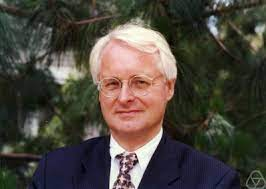
\includegraphics[scale = .5]{lenstra.jpeg}

\begin{itemize}[<+->]
\item Hendrik Lenstra Jr. recieved his doctorate from the University of Amsterdam in 1977.

\item Discovered Elliptic Curve Factorization (ECM) in 1987.

\item ECM is third-fastest known factoring algorithm and the best algorithm for finding divisors not exceeding 50-60 digits.

\item The largest factor found using ECM has 83 digits.
\end{itemize}
\end{frame}

\begin{frame}
\frametitle{Group Theory behind Pollard $p-1$}

\uncover<2->{$\textbf{Definition}$ Let $(G,+)$ be a group. If $H \subset G$ is also a group under $+$, then we call $H$ a subgroup of $G$. }

\uncover<3->{$\textbf{Lagrange's Theorem}$ If $H \subset G$ with $\vert G \vert < \infty$, then $\vert H\vert$ divides $\vert G \vert$. }

\begin{itemize}
\item<4-> Define the relation $a \sim b$ whenever $a = bh$ for some $h \in H$. 
\item<5-> Let $S$ be an equivalence class of $\sim$ and pick an arbitrary $a \in S$.
\item<6-> Define $f: S \rightarrow H$, where $f(b) = b^{-1}a$ and $g:H \rightarrow S$ by $g(h) = ah^{-1}$
\item<7-> Observe $f$ and $g$ are inverses.
$$f(g(h)) = f(ah^{-1}) = (ah^{-1})^{-1}a = h$$
$$g(f(b)) = g(b^{-1}a) = a(b^{-1}a)^{-1} = b$$
\item<7-> Thus, $\vert S \vert = \vert H \vert$ for all equivalence classes $S$.
\item<8-> Therefore, $\vert G \vert = n \vert H \vert$. 
\end{itemize}
\end{frame}

\begin{frame}
\frametitle{A different perspective} 
\uncover<2->{$\textbf{Lemma 2.2.5}$ Suppose that $m$, $n \in \mathbb{N}$ and gcd$(m,n) = 1$. Then the map
$$
    \psi : \left( \mathbb{Z}/mn\mathbb{Z} \right)^* \rightarrow \left( \mathbb{Z}/m\mathbb{Z} \right)^* \times \left( \mathbb{Z}/n\mathbb{Z} \right)^*
$$
defined by
$$
    \psi(c) = (c \pmod{m}, c\pmod{n})
$$
is a bijection.}
\end{frame}


\begin{frame}
\frametitle{Example}

\begin{itemize}
\item <2-> Let $B_i = \text{lcm}(1,\ldots, i)$.
\end{itemize}

\center
\begin{tabular}{c|c|c}
\uncover<3->{$B_i$} & \uncover<3->{$2^{B_i} \pmod{1763}} $& \uncover<3->{$(2^i \pmod{41}, 2^i \pmod{43})$} \\
\hline
\uncover<3->{1} & \uncover<3->{2} & \uncover<3->{(2,  2) }\\
\uncover<4->{2} & \uncover<4->{4} &  \uncover<4->{(4, 4 )}\\
\uncover<5->{6} &\uncover<5->{570} & \uncover<5->{(37, 11)} \\
\uncover<6->{60} & \uncover<6->{575} & \uncover<6->{(1, 16)}
\end{tabular}


\begin{itemize}
\item<6-> We compute $gcd(574, 1763) = 41$
\end{itemize}
\end{frame}

\begin{frame}
\frametitle{Set up for ECM}

\begin{itemize}
\item<2-> Let $E$ be an elliptic curve over $\mathbb{Z}/N\mathbb{Z}$ of the form
$$
	y^2 = x^3 + ax + 1
$$
such that $4a^3 + 27 \in \left(\mathbb{Z}/N\mathbb{Z}\right)^*$. This forces non singularity and ensures $P = (0,1)$ is on the curve.

\item<3-> Definition 6.3.1 (Power Smooth). Let $B$ be a positive integer. If $n$ is a positive integer with prime factorization
$$
    n = \prod p_i^{e_i},
$$
then $n$ is $B$-power smooth if $p_i^{e_i} \leq B$ for all $i$.

\item<4-> Example $30 = 2\cdot 3\cdot 5$ is $B$ power smooth for $B \geq 5$, but $150 = 2\cdot 3 \cdot 5^2$ is not $5$-power smooth.
\end{itemize}
\end{frame}

\begin{frame}
\frametitle{Motivation}

% Explain why p-1 not being B power smooth for a fixed B is a problem
\begin{itemize}
\item<2-> Fix $B \in \mathbb{N}$. Let $p \in \mathbb{N}$ such that $p-1$ is not $B$- power smooth.

\item<3-> Recall, in Pollard $p-1$, this would be equivalent to not having $p-1 \not \vert m = \text{lcm}(1,2, \ldots, B)$; i.e. $a^m \not \equiv 1 \pmod{p}$.

\item<4-> On the interval $[10^{15}, 10^{15} + 10000]$ 15 percent of the primes $p$ are such that $p-1$ is not $10^{6}$-power smooth.

\item<5-> The idea of ECM is to replace modular exponentiation on $\left(\mathbb{Z}/N\mathbb{Z}\right)^*$ by repeated addition of points on $E\left(\left(\mathbb{Z}/N\mathbb{Z}\right)^*\right)$

\item<6-> Recall, by the Hasse-Weil bound we can reduce the size of our group by $2\cdot \sqrt{p}$.
\end{itemize}
\end{frame}

\begin{frame}
\frametitle{Elliptic Curve Factorization}

Algorithm 6.3.10 (Elliptic Curve Factorization Method). Let $N$ and $B$ be positive integers.
\begin{itemize}
\item[1.]<2-> Compute $m =$ lcm$(1,2,\ldots, B)$.
\item[2.]<3-> Choose $a \in \mathbb{Z}/N\mathbb{Z}$ such that $4a^3 + 27 \in \left(\mathbb{Z}/N\mathbb{Z}\right)^*$. This forces $P = (0,1)$ to be a point on $y^2 = x^3 + ax +1$ over $\mathbb{Z}/N\mathbb{Z}$.
\item[3.]<4-> Try to compute $mP$. If at some point we cannot compute a sum of points, then some denominator $g$ is not coprime to $N$, then $gcd(g,N)$ is a nontrivial divisor of $N$.
\end{itemize}
\end{frame}

\begin{frame}
\frametitle{Analogy to Pollard $p-1$}
\begin{table}[h!]
  \begin{center}
    \uncover<2->{\caption{Let $E$ be an elliptic curve, and $m = lcm(1,2,\ldots,B)$ for some $B$}}
    \label{tab:table1}
    \begin{tabular}{|c|c|} % <-- Alignments: 1st column left, 2nd middle and 3rd right, with vertical lines in between
      \uncover<3->{\textbf{Pollard $p-1$} & \textbf{ECM}} \\
      \hline
      $\uncover<4->{\mathbb{Z}/N\mathbb{Z}$ & $E\left( \mathbb{Z}/N\mathbb{Z} \right)$}\\ &\\
      \uncover<5->{$g \in (\mathbb{Z}/N\mathbb{Z})^*$ & $(0,1)$} \\ & \\
       \uncover<6->{$g^m \equiv 1 \pmod{N}$ &  $mP \notin E\left( \mathbb{Z}/N\mathbb{Z} \right)$} \\ &\\
       \uncover<7->{$gcd(g^m-1, N)$ &  $gcd(m,N)$}
    \end{tabular}
  \end{center}
\end{table}

\begin{itemize}
\item<7-> If Pollard $p-1$ fails, we have no choice but to increase $B$.
\item<8-> However, ECM has a second option. We can choose another random elliptic curve.
\end{itemize}
\end{frame}


\begin{frame}
\frametitle{Why ECM "Works"}

\uncover<2->{We can consider an analogous mapping
$$
	"g: E(\mathbb{Z}/N\mathbb{Z}) \rightarrow \prod_{p\vert N} E(\mathbb{Z}/p\mathbb{Z})"
$$
where $p$ are prime divisors of $N$.}

\begin{itemize}
\item<3-> Note the quotations. There is a subtly in the difference between $E(\mathbb{Z}/N\mathbb{Z})$ and $\mathbb{Z}/N\mathbb{Z}$.
\end{itemize}
\end{frame}

\begin{frame}
\frametitle{Implementation}

\begin{itemize}
    \item Generate a random elliptic curve $E \pmod{N}$ and let $P = (0,1)$.
    \item Compute $m = lcm(1,2,...,B)$.
    \item Compute $mP$ (don't be naive!).
    \item If the calculation fails, you have found a non-trivial factor of $N$.
    \item Otherwise, just generate a new Elliptic curve and try again.
    % The calculation can sped up with $\ldots 3 \cdot (2 \cdot P)$.
    % \item Further optimization is possible using the Sieve of Eratosthenes (\texttt{prime\_range()}).
\end{itemize}

\end{frame}

\begin{frame}
\frametitle{Computing lcm(1,2,...,B)}

Recall,

\[ lcm(1,2,...B) = \prod_{p \in P} p^r \]

where $r = \text{max} \{ r \in \mathbb{Z} \mid p^r \leq B \}$.

\begin{align*}
    p^r &\leq B \\
    r\log(p) &\leq \log(B) \\
    r &\leq \log_p(B) \\
    r &= \lfloor \log_p(B) \rfloor \\
\end{align*}

\end{frame}

\begin{frame}

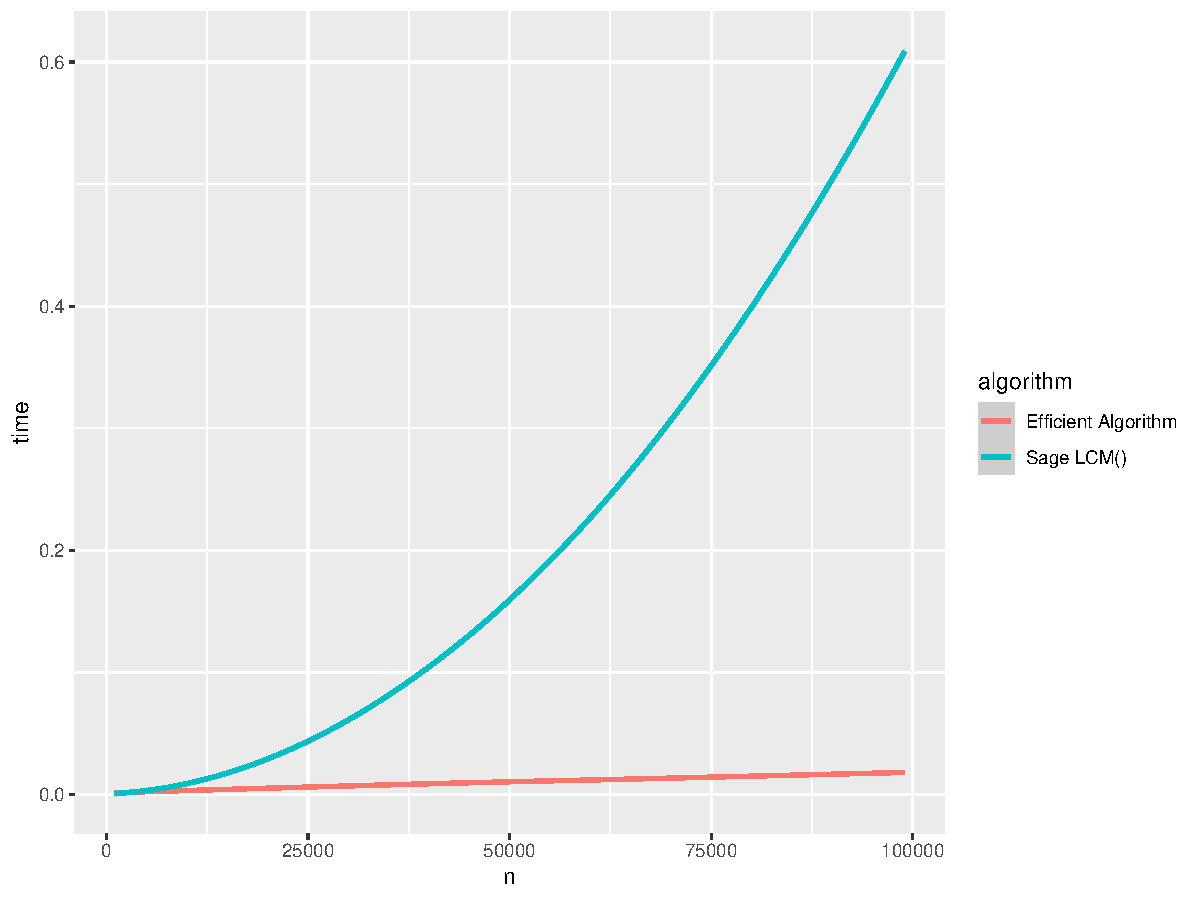
\includegraphics[width=\textwidth]{graphs/lcm_comparison.pdf}

\end{frame}

\begin{frame}
\frametitle{Computing $mP$}

\[ mP = \overbrace{P + P + P \ldots P}^\text{$m$ times} \]
\begin{center}
    A very bad way to compute $mP$.
\end{center}

There are many algorithms for computing general elliptic curve point multiplication efficiently, but given the very specific make-up of $m$, we can save time by being thoughtful here.

Consider,

\[ m_n = q_1^{r_1} \cdot q_2^{r_2} \ldots q_n^{r_n} \]

then

\[ m_nP = q_n^{r_n} \cdot m_{n-1}P \]

\end{frame}

\begin{frame}

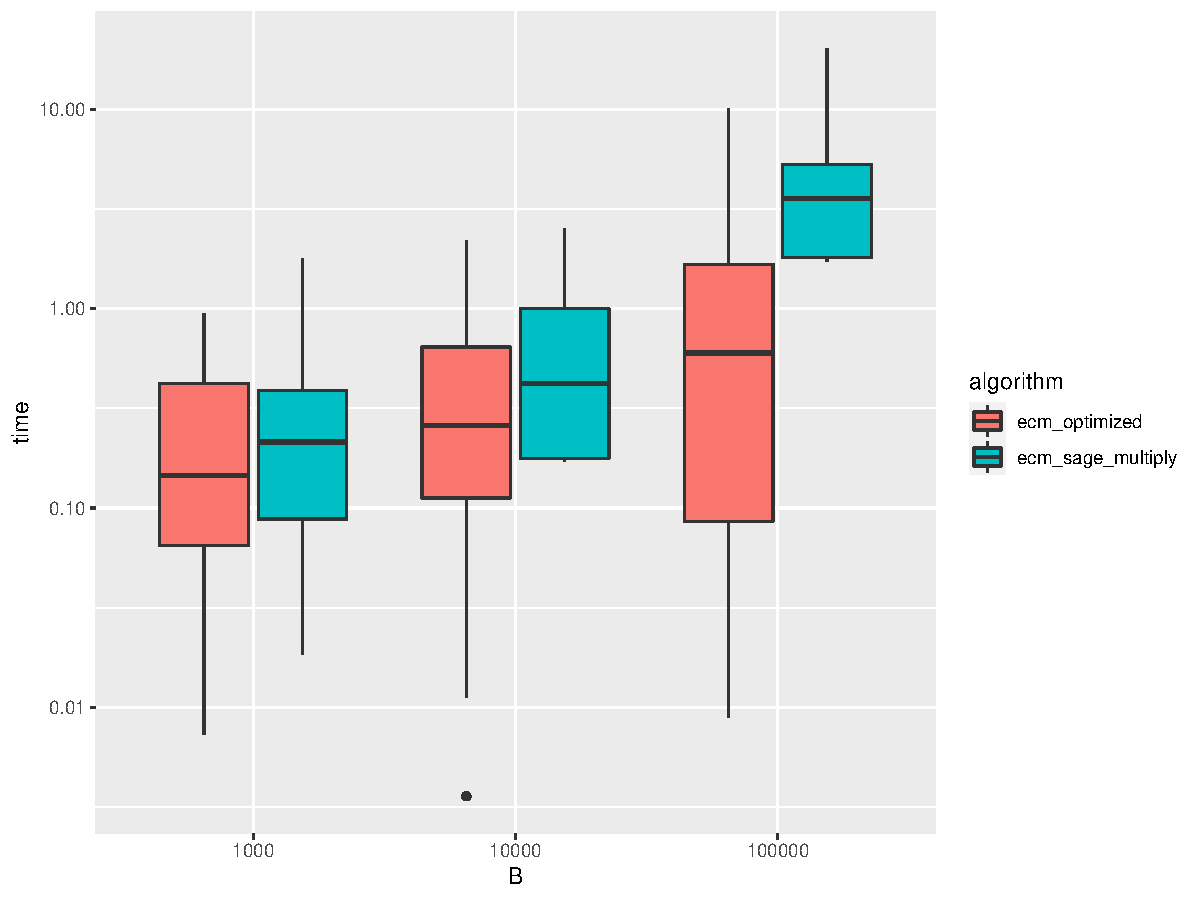
\includegraphics[width=\textwidth]{graphs/ecm_perf.pdf}

\end{frame}

\begin{frame}
\frametitle{Coded Example}

\lstinputlisting[language=Python]{ecm.sage}

\end{frame}

\begin{frame}
\frametitle{Animation}

\end{frame}

\end{document}
